\documentclass[10pt]{beamer}
\usepackage{amsmath}
\usepackage{amssymb}
\usepackage{geometry}
\usepackage{graphicx}
\usepackage{url}
\usepackage{bm}

\makeatletter
\let \@sverbatim \@verbatim
\def \@verbatim {\@sverbatim \verbatimplus}
{\catcode`'=13 \gdef \verbatimplus{\catcode`'=13 \chardef '=13 }} 
\makeatother

\begin{document}

%-------------------------------------------
\begin{frame}
\large
Lecture 5:\\ 
Transformations for Simple Linear Regression\\
STAT 632, Spring 2020
\end{frame}

%-------------------------------------------
\begin{frame}
Transformations can be used to
\vspace{5pt}
\begin{itemize}
\item Linearize the relationship between the explanatory ($X$) and response ($Y$) variables
\vspace{5pt}
\item Overcome problems due to nonconstant variance
\end{itemize}
\end{frame}

%-------------------------------------------
\begin{frame}{Example: Modeling Brain Weight}
\begin{itemize}
\item We consider a data set called \texttt{brains} from the \texttt{alr4} package.  The data set is on the the brain weight (in grams) and body weight (in kg)  for 62 species of mammals.
\vspace{5pt}
\item A scatter plot of the data (next slide) shows that the variables are extremely skewed. Three points (humans and two species of elephants) stand out from the rest of the data.
\end{itemize}
\end{frame}

%-------------------------------------------
\begin{frame}[fragile]
\small
\begin{verbatim}
> library(alr4) 
> plot(BrainWt ~ BodyWt, data=brains)
\end{verbatim}
\begin{figure}
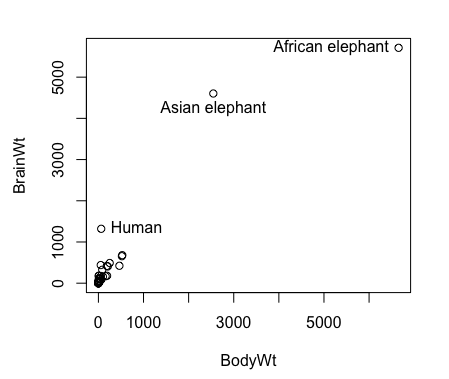
\includegraphics[scale=0.4]{figure/brainplot.png}
\end{figure}
\end{frame}

%-------------------------------------------
\begin{frame}
The histograms illustrate that the log transformation can reduce the positive skew in the data.
\begin{figure}
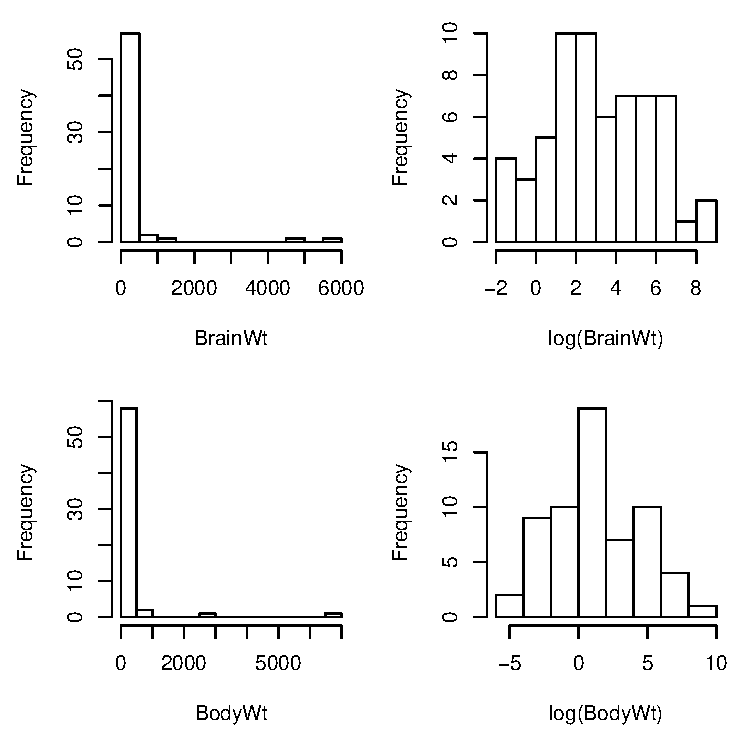
\includegraphics[scale=0.5]{figure/brain_hist.pdf}
\end{figure}
\end{frame}

%-------------------------------------------
\begin{frame}[fragile]
The log transformation linearizes the relationship between the variables.
\small
\begin{verbatim}
> lm1 <- lm(log(BrainWt) ~ log(BodyWt), data=brains)
> plot(log(BrainWt) ~ log(BodyWt), data=brains)
> abline(lm1)
\end{verbatim}
\begin{figure}
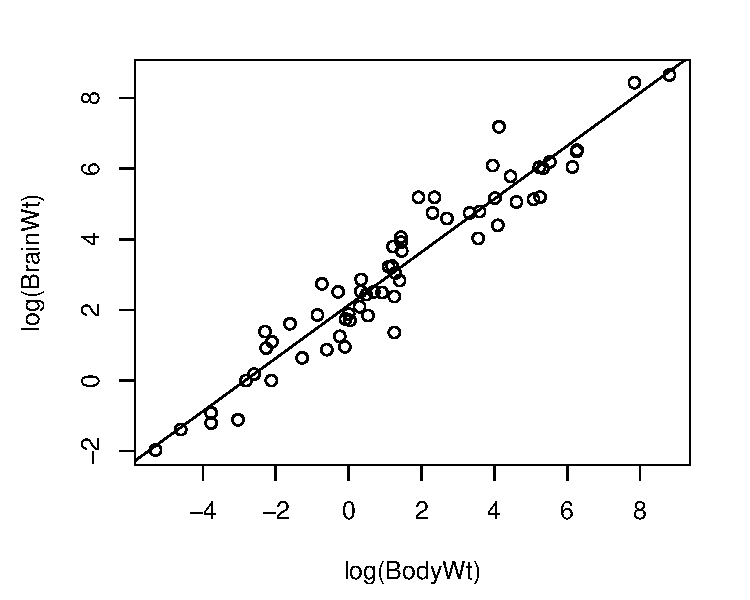
\includegraphics[scale=0.5]{figure/logbrain_scat.pdf}
\end{figure}
\end{frame}

%-------------------------------------------
\begin{frame}[fragile]
After taking the log transformation, the residual plot shows no discernible patterns (random scatter of points around 0).  The assumptions of linearity and constant variance appear to be well satisfied.
\small
\begin{verbatim}
> plot(predict(lm1), resid(lm1), xlab='Fitted values', ylab='Residuals')
> abline(h=0, lty=2)
\end{verbatim}
\begin{figure}
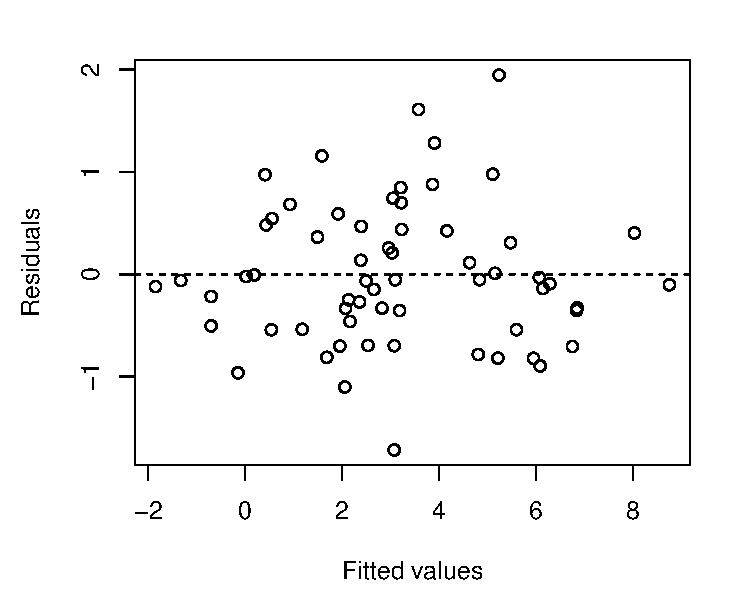
\includegraphics[scale=0.5]{figure/logbrain_resid.pdf}
\end{figure}
\end{frame}

%-------------------------------------------
\begin{frame}[fragile]
\small
\begin{verbatim}
> summary(lm1)
Coefficients:
            Estimate Std. Error t value Pr(>|t|)    
(Intercept)  2.13479    0.09604   22.23   <2e-16 ***
log(BodyWt)  0.75169    0.02846   26.41   <2e-16 ***
---
Signif. codes:  0 ‘***’ 0.001 ‘**’ 0.01 ‘*’ 0.05 ‘.’ 0.1 ‘ ’ 1

Residual standard error: 0.6943 on 60 degrees of freedom
Multiple R-squared:  0.9208,	Adjusted R-squared:  0.9195 
F-statistic: 697.4 on 1 and 60 DF,  p-value: < 2.2e-16
\end{verbatim}
\end{frame}

%-------------------------------------------
\begin{frame}
The R output gives the following regression equation:
\begin{align*}
\widehat{\log(\texttt{BrainWt})} &= \hat{\beta}_0 + \hat{\beta}_1 \log(\texttt{BodyWt})\\
& = 2.135 + 0.7517 \log(\texttt{BodyWt})
\end{align*}
\vspace{2.5pt}

%-------------------------------------------
\begin{itemize}
\item The interpretation of the estimated slope is that a unit increase in \texttt{log(BodyWt)} is associated with an increase in \texttt{log(BrainWt)} by 0.7517 (not that useful).  
\vspace{5pt}
\item Another common interpretation is in terms of percentage effects: A 1\% increase in body weight (kg) is associated with an approximate 0.75\% increase in brain weight.\footnote{See Sheather, Section 3.3.2, pp.79-80, for a mathematical explanation}
\end{itemize}
\end{frame}

%-------------------------------------------
\begin{frame}{Review of logs}
\begin{itemize}
\item Logs are exponents: $\log_b(x) = y$ (read ``the log of $x$ to the base $b$ is $y$") means that $b^y = x$.  Some examples:
\begin{align*}
\log_{10} 100 = 2 &\Longleftrightarrow 10^2 = 100\\
\log_{10} 0.01 = -2 &\Longleftrightarrow 10^{-2} = 0.01\\
\log_{2} 8 = 3 &\Longleftrightarrow 2^3 = 8
\end{align*}
\item Some useful identities:
\begin{align*}
e^{\log(x)} &= x\\
\log(x^r) &= r \log(x)\\
\log(xy) &= \log(x) + \log(y)\\
\log(x/y) &= \log(x) - \log(y)
\end{align*}
\end{itemize}
Note: $\log(x)$ denotes the log base $e$ here (this is called the natural logarithm, which is also commonly denoted by $\ln(x)$)
\end{frame}

%-------------------------------------------
\begin{frame}
\vspace{-3.5cm}
 We can back-transform to write the model in the original scale of the response.  
% \begin{align*}
% e^{\widehat{\log(\texttt{BrainWt})}} &=   e ^{\hat{\beta}_0 + \hat{\beta}_1 \log(\texttt{BodyWt})}\\
% \widehat{\texttt{BrainWt}} & = e ^{\hat{\beta}_0}  e^{\hat{\beta}_1 \log(\texttt{BodyWt})}\\
%  & = e ^{\hat{\beta}_0}  e^{\log(\texttt{BodyWt}^{\hat{\beta}_1 })}\\
% &= \hat{\alpha} \cdot \texttt{BodyWt}^{\hat{\beta}_1 }
% \end{align*}
% Plugging in the estimates gives:
% $$\widehat{\texttt{BrainWt}} = 8.455 \cdot \texttt{BodyWt}^{0.7517}$$
% 
% This is often referred to as a \textbf{power-law} relationship.\footnote{\url{https://en.wikipedia.org/wiki/Power_law}}
\end{frame}

%-------------------------------------------
\begin{frame}
Regression equation for $\log(\texttt{BrainWt})$:
$$\widehat{\log(\texttt{BrainWt})}= 2.135 + 0.7517 \log(\texttt{BodyWt})$$\\
\vspace{5pt}

Make a prediction for $\log(\texttt{BrainWt})$ when \texttt{BodyWt} is 40 kg:
$$\widehat{\log(\texttt{BrainWt})} = 2.135 + 0.7517 \log(40) = 4.908$$\\
\vspace{5pt}

We can then exponentiate both sides to get the prediction for \texttt{BrainWt} (in grams) when when \texttt{BodyWt} is 40 kg:\\
$$\widehat{\texttt{BrainWt}} = e^{4.908} = 135.37$$
\end{frame}

%-------------------------------------------
\begin{frame}[fragile]
\begin{verbatim}
# use R to make prediction for log(BrainWt) when BodyWt is 40
> pred <- predict(lm1, data.frame(BodyWt = 40), 
                  interval="prediction")
> pred
       fit      lwr      upr
1 4.907668 3.501332 6.314003


# exponentiate to make prediction for BrainWt
> exp(pred)
       fit      lwr      upr
1 135.3235 33.15961 552.2514
\end{verbatim}
\end{frame}

%-------------------------------------------
\begin{frame}{Summary: Log Transformation}
A log transformation might be useful if
\begin{itemize}
\item the distribution of the response or predictor variable is skewed right.
\item the values of the variable range over more than one order of magnitude.
\item there is a fan pattern in the residuals (nonconstant variance).
\end{itemize}
\vspace{15pt}

\textbf{Remark}: The transformation $log(x_i)$ is only valid for $x_i>0$.  For nonpositive data, one workaround is to use the transformation $log(x_i + c)$, where $c$ is a constant such that $x_i + c > 0$, for $i=1,\cdots,n$.  
\end{frame}

%-------------------------------------------
\begin{frame}[fragile]{Example: Doctors and Hospitals} 
Data set containing counts on the number of medical doctors and number of hospitals in a random sample of 53 counties. 
\begin{verbatim}
> library(Stat2Data)
> data("CountyHealth")
> head(CountyHealth)
County              MDs Hospitals Beds
1 Bay, FL           351         3  605
2 Beaufort, NC       95         2  134
3 Beaver, PA        260         2  567
4 Bernalillo, NM   2797        11 1435
5 Bibb, GA          769         5  976
6 Clinton, PA        42         2  245
\end{verbatim}
\end{frame}

%-------------------------------------------
\begin{frame}[fragile]
\begin{verbatim}
> lm1 <- lm(MDs ~ Hospitals, data = CountyHealth)
> plot(MDs ~ Hospitals, data = CountyHealth)
> abline(lm1)
\end{verbatim}
\begin{figure}
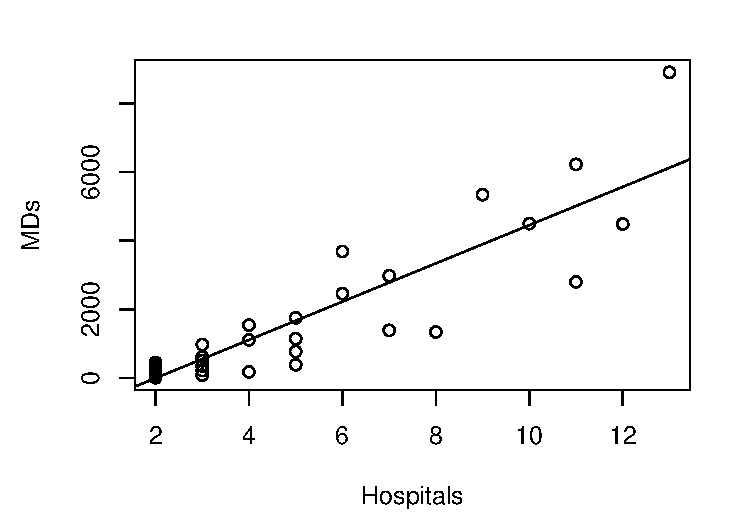
\includegraphics[scale=0.6]{figure/MDs_scatter1.pdf}
\end{figure}
\end{frame}

%-------------------------------------------
\begin{frame}[fragile]
There residual plot shows nonconstant variance.  That is, the variability in the residuals tends to increase with the fitted values.  The QQ plot also indicates that the residuals deviate from a normal distribution.
\small
\begin{verbatim}
> par(mfrow = c(1, 2))
> plot(lm1, 1:2)
\end{verbatim}
\begin{figure}
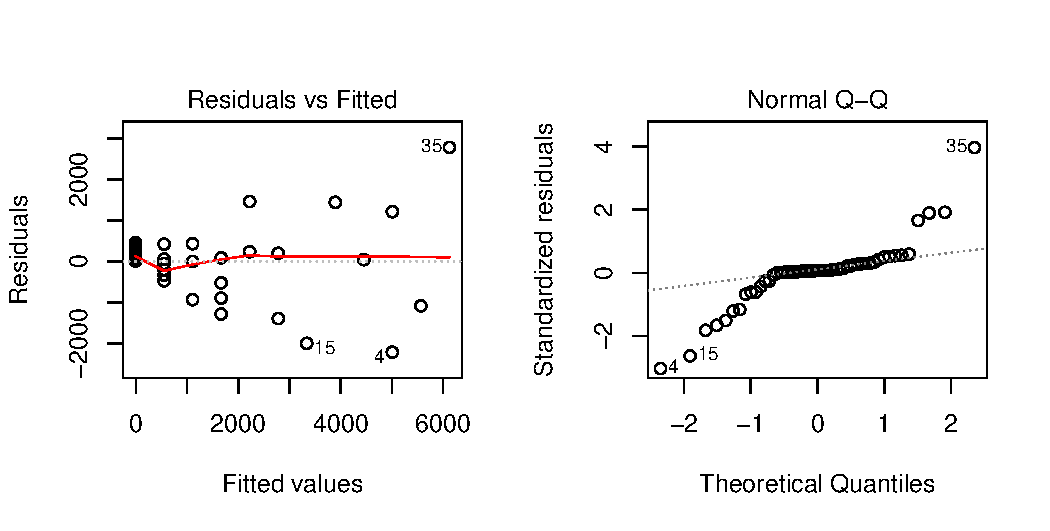
\includegraphics[scale=0.55]{figure/diagnostic1.pdf}
\end{figure}
\end{frame}

%-------------------------------------------
\begin{frame}{Using Transformations to Stabilize Variance}
\begin{itemize}
\item Problems with nonconstant variance can be overcome with transformations.
\vspace{5pt}
\item Two common variance stabilizing transformations are the log transformation, $\log(Y)$, and the square root transformation, $\sqrt{Y}$.  
\vspace{5pt}
\item The square root transformation is often appropriate for count data.
\vspace{5pt}
\item Since the data in this example are in the form of counts, we will try a square root transformation of the response.  
% \item Note that, when $X$ and $Y$ are both measured in the same units it is recommended to consider the same transformation for both variables.
\end{itemize}
\end{frame}

%-------------------------------------------
\begin{frame}[fragile]
\begin{verbatim}
lm2 <- lm(sqrt(MDs) ~ Hospitals, data = CountyHealth)
plot(sqrt(MDs) ~ Hospitals, data = CountyHealth)
abline(lm2)
\end{verbatim}
\begin{figure}
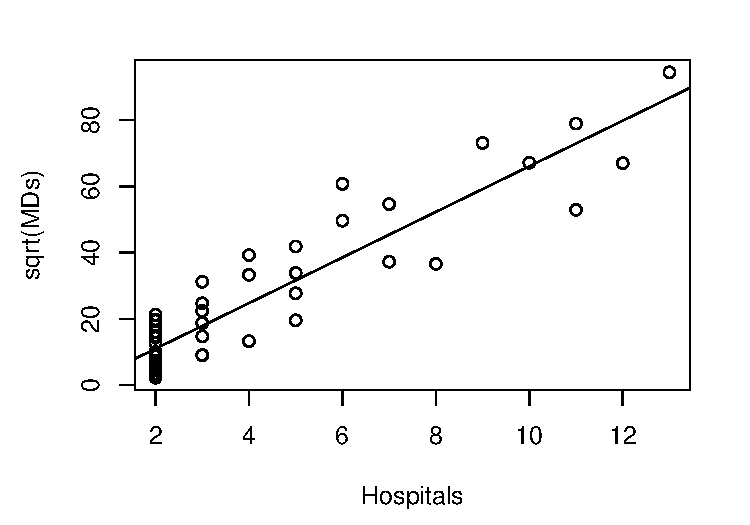
\includegraphics[scale=0.6]{figure/MDs_scatter2.pdf}
\end{figure}
\end{frame}

%-------------------------------------------
\begin{frame}[fragile]
Afre taking the square root transformation, the residual plot and QQ plot show considerable improvement.  The assumptions of constant variability and normality in the residuals appear reasonably satisfied.
\begin{verbatim}
> par(mfrow = c(1, 2))
> plot(lm2, 1:2)
\end{verbatim}
\begin{figure}
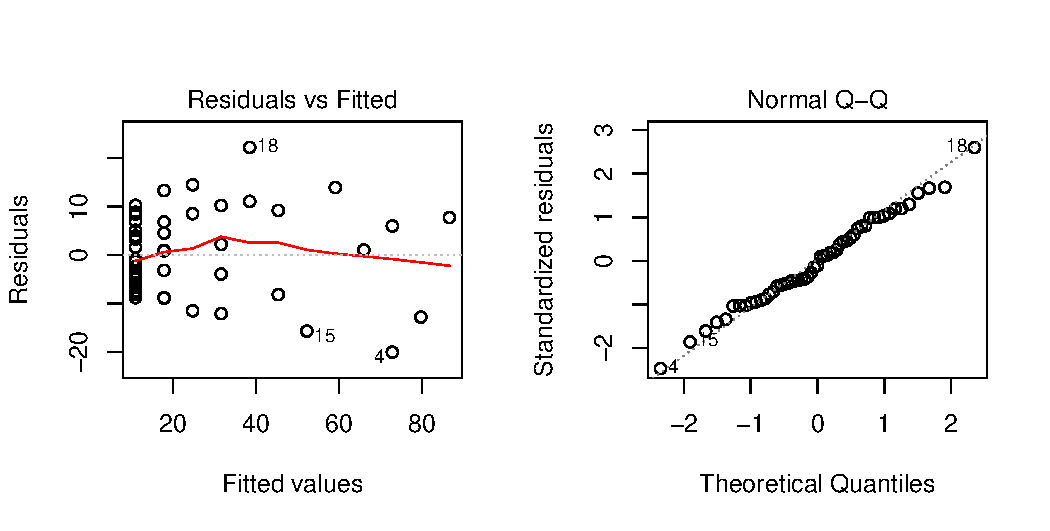
\includegraphics[scale=0.55]{figure/diagnostic2.pdf}
\end{figure}
\end{frame}

%-------------------------------------------
\begin{frame}[fragile]
\begin{verbatim}
> summary(lm2)
Coefficients:
            Estimate Std. Error t value Pr(>|t|)    
(Intercept)  -2.7533     1.9850  -1.387    0.171    
Hospitals     6.8764     0.4011  17.144   <2e-16 ***
\end{verbatim}
\vspace{10pt}

Regression equation for the transformed model:
$$\widehat{\sqrt{\texttt{MDs}}} = -2.7533 + 6.8764 \, \texttt{Hospitals}$$

We can back-transform to write the model in the original scale of the response. 
$$\widehat{\texttt{MDs}} = (-2.7533 + 6.8764 \, \texttt{Hospitals})^2$$
\end{frame}
% Make prediction for specific value in R


%-------------------------------------------
\begin{frame}{Summary}
\begin{itemize}
\item It can take some trial and error to find a good transformation.  Looking at scatterplots of the data and residuals can help determine which transformation best linearizes the relationship or stabilizes the variance.
\item The log transform is commonly applied to skewed data that ranges over several orders of magnitude.
\item The square root transform is commonly applied to count data to stabilize the variance.
\item Transformations can be applied to the response variable, explanatory variable(s), or both. 
\item Transforming the response can make the model more difficult to interpret.  Predictions and prediction intervals need to be back-transformed so that they can be interpreted on the original scale.
\end{itemize}
\end{frame}



\end{document}